% ICCS'09 http://www.iccs-meeting.org/iccs2009/}
% svn co https://svn.mcs.anl.gov/repos/performance/orio/doc/papers/iccs09
% Important dates:
% Full papers submission (extended)       December 20, 2008
% Notification of acceptance of papers    February 2, 2009
% Camera ready papers                        February 15, 2009
% Max 10 pages, llncs style

\documentclass[runningheads]{llncs}

\usepackage{amssymb}
\setcounter{tocdepth}{3}
\usepackage{graphicx}
\usepackage{url}
\usepackage{html}
\usepackage{subfigure}
\usepackage{cite}
\usepackage{wrapfig}
\usepackage{amsmath}

\urldef{\mailsa}\path|{alfred.hofmann,ursula.barth,ingrid.beyer,natalie.brecht,|
\urldef{\mailsb}\path|christine.guenther,frank.holzwarth,piamaria.karbach,|
\urldef{\mailsc}\path|anna.kramer,erika.siebert-cole,lncs}@springer.com|
\newcommand{\keywords}[1]{\par\addvspace\baselineskip
\noindent\keywordname\enspace\ignorespaces#1}

\newenvironment{itemizer}{\begin{itemize}\setlength{\parsep}{0cm}\setlength{\itemsep}{-.3em}}{\end{itemize}}

% formatting cheats
%\renewcommand{\baselinestretch}{0.92}  
%\renewcommand\floatpagefraction{.9} 
%\renewcommand\topfraction{.9} 
%\renewcommand\bottomfraction{.9} 
%\renewcommand\textfraction{.1} 
%\setcounter{totalnumber}{50} 
%\setcounter{topnumber}{50} 
%\setcounter{bottomnumber}{50} 
%\setlength{\textwidth}{12.5cm} 
%\setlength{\textheight}{19.5cm} 


\begin{document}

\mainmatter  % start of an individual contribution

% first the title is needed
\title{Generating Empirically Optimized Composed Matrix Kernels from MATLAB Prototypes}

        % a short form should be given in case it is too long for the running head
        \titlerunning{Empirically Optimized Numerical Software from MATLAB}

\author{Boyana Norris\thanks{The work of this author was supported by the Office of Advanced Scientific Computing Research, Office of Science, U.S. Dept. of Energy, under Contract DE-AC02-06CH11357.}\inst{1}
  \and Albert Hartono\inst{2}
  \and Elizabeth Jessup\thanks{The work of this author was supported by the
  National Science Foundation under grants no. CCF-0430646 and CCF-830458.}\inst{3}
  \and Jeremy Siek\inst{3}
%
\authorrunning{Norris, Hartono, Jessup, Siek}
%
\institute{Argonne National Laboratory \\
  \email{norris@mcs.anl.gov}
  \and Ohio State University \\
  \email{hartonoa@cse.ohio-state.edu}
  \and University of Colorado at Boulder \\
  \email{\{elizabeth.jessup,jeremy.siek\}@colorado.edu}}}

\tocauthor{B. Norris, A. Hartono, E. Jessup, and J. Siek}
\maketitle

\begin{abstract}
% between 75 and 150 words
%The growing demand for higher levels of detail and accuracy in results means
%that the size and complexity of scientific computations is increasing at
%least as fast as the improvements in processor technology. 
%Programming
%scientific applications is hard, and optimizing them for high performance is
%even harder.  
The development of optimized codes is time-consuming and requires extensive
architecture, compiler, and language expertise; therefore, computational
scientists are often forced to choose between investing too much time in
tuning code or accepting lower performance.
%
In this paper, we describe the first steps toward a fully automated system
for the optimization of the matrix algebra kernels that are a foundational
part of many scientific applications.  To generate highly optimized code from
a high-level MATLAB prototype, we define a three-step approach.  To begin, we
have developed a compiler that converts a MATLAB script into simple C code.
We then use the polyhedral optimization system PLuTo to optimize that code
for coarse-grained parallelism and locality simultaneously. Finally, we
annotate the resulting code with performance tuning directives and use the
empirical performance tuning system Orio to generate many tuned versions of
the same operation using different optimization techniques, such as loop
unrolling and memory alignment. Orio performs an automated empirical search
to select the best among the multiple optimized code variants. We discuss
performance results on two architectures.
%showing that the code generated by using our system
%significantly outperforms not only the original simple C code but also code
%based on source BLAS, ATLAS-optimized BLAS, and Intel MKL routines.
\keywords{Code generation, empirical performance tuning}
\end{abstract}



\section{Introduction}
\label{sec:intro}

The development of high-performance numerical codes is challenging because
performance is determined by complex interactions among the algorithm, data
structure, programming language, compiler, and computer
architecture. Scientists seeking high performance are thus required to master
advanced concepts in computer science and carry out intricate programming
tasks in addition to managing the scientific content of their work.  They
must either invest substantial time in tuning their software or accept low
performance. In either case, the productivity of the scientists degrades.

Historically, the research community has pursued two separate paths toward
the goal of making software run at near-peak levels.  The first path builds
on research into compilers and their associated technologies.  One of the
main goals of compilation research is to take an arbitrary code as input and
produce optimal code as output for a given language and hardware platform.
The success of this approach has been limited by a number of factors: (i)
optimal mappings between the computation graph and the hardware are expensive
(often NP-complete) to compute; (ii) potentially useful information that
could aid optimization cannot be represented in general-purpose languages
such as C and Fortran; and (iii) user control of compiler optimizations is
limited and varies from compiler to compiler, and (iv) apart from differences
in execution time, it is difficult to evaluate the effectiveness of
different compiler optimizations.

When compilers alone cannot achieve the desired performance, 
another path to performance optimization is to identify kernel
routines that dominate the execution time of a wide variety of
applications.  
%When such kernels can be identified and agreed upon by the
%members of the community, programmers with the required level of technical
%knowledge can concentrate on producing these optimized kernel libraries for
%architectures of interest. 
An example is the high-performance Basic Linear Algebra Subprograms 
(BLAS) libraries~\cite{BLAS} produced by a combination
of hardware vendors, independent software vendors, and researchers.
Developers who write their codes calling these routines can achieve high
performance across all supported architectures, but are also subject to 
the limitations of the library (e.g., portability and the types of operations available).
%The efforts in
%high-performance library development aptly demonstrate, however, that the
%research into compiler technologies has not been fully successful.  If
%compilers could take the relatively simple code such as a dense matrix-matrix
%product and produce optimal code, this second approach would be unnecessary.
%Like compiler optimization, the kernel library-oriented approach has
%significant limitations.  Support for a variety of architectures is the most
%serious problem because the optimizations necessary to achieve near-peak
%performance are by nature not portable, requiring manual update or
%reimplementation for each new architecture.

This paper describes a combination of the two approaches designed to overcome
some of their shortcomings. We describe our initial efforts toward the
development of software infrastructure for \emph{generating} automatically
tuned libraries for matrix algebra computations.  In
Section~\ref{sec:background} we briefly discuss relevant prior and current
research efforts. In Section~\ref{sec:approach} we describe our
MATLAB-to-C compiler and the empirical performance
tuning system Orio and its use in conjunction with the Pluto tool suite to
generate and empirically evaluate many tuned versions of the C code generated
by the MATLAB compiler.  In Section~\ref{sec:experiments} we provide
performance results on two architectures. In Section~\ref{sec:conclusion} we conclude 
with a brief summary.

\section{Background}
\label{sec:background}

Existing optimizing MATLAB~\cite{matlab:webpage} compilers, such as the MaJIC
MATLAB compiler~\cite{MaJIC}, include limited local optimizations for matrix
expressions but do not perform optimizations such as loop fusion across
multiple operations as we do with the tools described in this paper. The
telescoping languages
%~\cite{telescopingurl,teleoverview,Ken99} 
project~\cite{telescopingurl} uses techniques such as
strength reduction, vectorization, and procedure specialization to optimize
MATLAB scripts but does not generate reusable optimized linear algebra
routines as described in this paper.

The most common approach to tuning numerical codes is for an expert to
transform the source manually, unrolling loops, blocking for multiple levels
of cache, and inserting prefetch instructions.  The pitfalls of this approach
are well understood~\cite{Goedecker01}: It requires a significant amount of
time and effort. Optimizing code for one particular platform may in fact make
it less efficient on other platforms and often makes it complex and hard to
understand or maintain.  An alternative is the use of tuned libraries of key
numerical algorithms, for example, BLAS~\cite{Dongarra:1990fk} and
LAPACK~\cite{LAPACK} for dense linear algebra.
%, SPARSPAK~\cite{sparspak} for
%sparse linear algebra, and BLITZ++~\cite{blitz} to support scientific
%computing in C++, or GPULib by Tech-X, an open source library for
%accelerating numerical computations on Graphics Processing
%Units~\cite{gpulib}, to name just a few). Such libraries are difficult to
%develop, and they generally cannot adapt to execution context: as we note in
%Section~\ref{sec:approach}, a series of calls to library routines can incur
%high memory costs.

Specialized code generators circumvent the high costs of manual code
generation. They include tools for basic dense linear algebra operations
(ATLAS~\cite{WN147}, PhiPAC~\cite{bilmes97optimizing}),
%,phipacwww})
and sparse linear algebra (OSKI~\cite{vuduc05})
%FFTs~\cite{FFTW,Spiral}), stencil-based
%
%operations~\cite{kamil06}, and tensor computations (TCE~\cite{TCE}) among
among others.  While these libraries target a specific kernel, our approach aims 
at enabling the definition of arbitrary kernels involving dense matrix linear algebra.
It is often impossible to predict precisely the performance of code
on modern computer architectures. Thus, many of these specialized code
generators exploit search strategies to identify the best (or nearly best)
code for a particular choice of problem parameters and machine. Most existing
autotuning tools are not general but focus on a specific domain or algorithm.
%While not all applications can be written in terms of available libraries,
%the performance achieved with autotuning tools does convincingly demonstrate
%the benefits of automated source code transformations.

%The best performance today is obtained through approaches like that taken by
%PERI~\cite{PERI} which involves a labor intensive rewrite of portion of the
%code by a group of performance tools experts in collaboration with
%application scientists. Maintaining performance of the code as the
%application and hardware evolves means that the tuning process may need to be
%repeated. Our efforts aim to capture this performance tuning expertise in a
%way that can be integrated into the application. We will thus enable
%performance portability and ensure that the improvements to the application
%are long-lasting.

A number of source or binary transformation tools for general
performance-improving optimizations exist. LoopTool~\cite{LoopTool},
developed at Rice University, supports annotation-based loop fusion,
unroll-and-jam, skewing, and tiling.  A relatively new tool, POET~\cite{POET},
also supports a number of loop transformations. POET offers a complex
template-based syntax for defining transformations in a language-independent
manner (but currently only C++ is supported). 
%Other recent research efforts whose goal, at least in part, is to
%enable optimizations of source code to be augmented with performance-related
%information include the X language~\cite{XLanguage} (a macro C-like language
%for annotating C code), the Broadway~\cite{broadway} compiler, and various
%meta-programming
%~\cite{veldhuizen95,weise93,kiczales91,chiba95}
%techniques (e.g., ~\cite{veldhuizen95,chiba95}). 
Pluto~\cite{Pluto}
%uday08cc} 
is a source-to-source transformation tool for
optimizing sequences of nested loops. Pluto employs a polyhedral model of
nested loops, where the dynamic instance (iteration) of each statement is
viewed as an integer point in a well-defined space, called the statement's
polyhedron. Combined with a characterization of data dependences, this
representation allows the construction of mathematically correct complex loop
transformations. The transformations target both improved cache locality and
parallelism.

\section{Optimizing Composed BLAS Operations}
\label{sec:approach}

Codes based on matrix algebra are generally constructed as a sequence of
calls to the BLAS
%~\cite{Dongarra:1988uq,Lawson:1979kx,Dongarra:1990fk} 
and similar
sparse matrix libraries~\cite{Saad:fr}.
%,George:1981uq}. 
Writing programs in
this way promotes readability and maintainability but can be costly in terms
of memory efficiency. Specifically, the retrieval of a large-order matrix at
each routine call can profoundly affect performance even when highly
tuned implementations of the BLAS (e.g.,~\cite{Goto:2006fk})
%(e.g.~\cite{Bilmes:1997ye,Whaley:1998fk,IntelMath:oq,ESSL:kl,Goto:2006fk})
are used.

A much more efficient approach is to call a single, specialized routine that
performs multiple operations, rather than to make successive calls to separate BLAS
routines (e.g., see ~\cite{gropp01}).
%~\cite{Ashby:uq,Blackford:2002vn,baker03blgmres,baker03lgmres,Dennis:2005tg,Howell:2008,gropp01,Vuduc:2003kl}.
Single routines that carry out more than one linear algebra operation are
known as \emph{composed} BLAS. As an example, consider the pair of
matrix-vector products $q = Ap$, $s = A^Tr$, where $A$ is a matrix and $p$,
$q$, $r$, and $s$ are vectors, that represent the computational bottlenecks
of the biconjugate gradient method (BiCG)~\cite{Saad:2003fk} and of the
GEMVER kernel examined in Section~\ref{sec:matlab}.  These two operations can
be implemented as a pair of calls to the BLAS routine {\tt GEMV}, or they can
be rewritten as a composed BLAS consisting of a doubly nested loop
encompassing both matrix-vector products. In the former case, the matrix $A$
is accessed twice, whereas in the latter it is accessed only once. Our
preliminary results in prior research and in the work reported in this paper
indicate that loop fusion leads to a routine that delivers significantly
better performance than does a pair of calls to the best optimized BLAS {\tt
GEMV} routines for large matrix orders.  Composed routines are the focus of
the work presented here, but much of what we discuss generalizes to a much
broader array of computations.

To generate highly optimized code from a MATLAB prototype of the composed
BLAS operation, we follow a three-step approach, illustrated in
Fig.~\ref{fig:process}.  This process is repeated when the MATLAB code changes
or the code must be tuned on a new architecture.
To begin, we have developed a compiler that
%
\begin{wrapfigure}{r}{3in}
\vspace{-.2in}
\centering
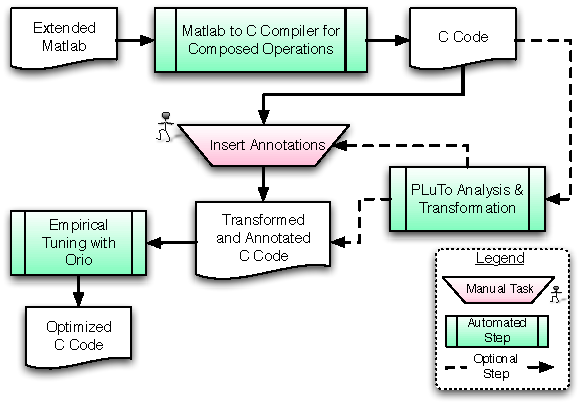
\includegraphics[width=3in]{figures/process.pdf}
\vspace{-.15in}
\caption{Code generation and tuning process.}
\label{fig:process}
\vspace{-.1in}
\end{wrapfigure}
%
converts a MATLAB script into simple C code~\cite{Siek}.  After generating
the C code from the high-level MATLAB prototype, we (optionally) use 
the source-to-source automatic parallelization tool Pluto~\cite{Pluto} %developed at Ohio State University
to optimize for coarse-grained parallelism and locality simultaneously. Using
the results of the Pluto analysis, we insert annotations into the C code,
which are then processed by our extensible annotation system Orio to generate
many tuned versions of the same operation using different optimization
parameters. Orio then performs an empirical search to select the best among
the multiple optimized code variants.

%Probably need some words about WHY this multipronged approach is a good idea.

In the remainder of this section we describe each of the tools developed by
the authors of this paper, namely, the MATLAB-to-C compiler~\cite{Siek} and the Orio
empirical tuning tool~\cite{Norris:2007,Hartono:IPDPS09}.

%\vspace{-.2in}
\subsection{A MATLAB Compiler}
\label{sec:matlab}

Figure~\ref{fig:compiler} gives an overview of the MATLAB-to-C compilation process~\cite{Siek}. 
The MATLAB kernel specification is parsed into a high-level intermediate
representation in the form of a dataflow graph, in which each node represents
a parameter (e.g., a scalar, matrix, or vector variable) of the kernel or an operation.
%
\begin{wrapfigure}{r}{2in}
%\vspace{-.2in}
\centering
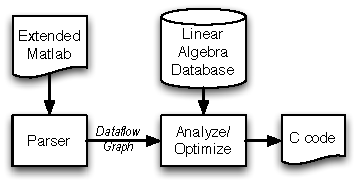
\includegraphics[width=2in]{figures/compile.pdf}
\caption{MATLAB-to-C compiler.}
\label{fig:compiler}
\vspace{-.2in}
\end{wrapfigure}
%
This dataflow graph is then iteratively processed until all of
the implementation choices have been made.  The compilation process consists
of three phases -- analysis, refinement, and optimization -- that are together
iterated until all of the implementation decisions have been made.  The graph
is then translated into C code.

%\subsubsection{The Dataflow Graph.}
%
%An example dataflow graph for the GEMVER kernel, defined below, is shown
%in Figure~\ref{fig:gemver-dataflow}.
%Each node represents a parameter of the kernel or an operation.  The arrows
%indicate the flow of data. At first the graph specifies what operations are
%to be performed but does not contain any implementation details. The symbol
%$\times$ in the depicted graph stands variously for outer product,
%matrix-vector multiplication, and scalar-vector multiplication, and it does
%not yet specify, for example, whether the outer products compute a row or a
%column at a time of the result matrix.
%\begin{figure}[ht]
%\begin{minipage}{.3\textwidth}
%\begin{align*}
%  A &\gets A + u_1 v_1^T + u_2 v_2^T \\[-0.5ex]
%  x &\gets \beta A^T y + z \\[-0.5ex]
%  w &\gets \alpha A x
%\end{align*} 
%\end{minipage}
%\begin{minipage}{.6\textwidth}
%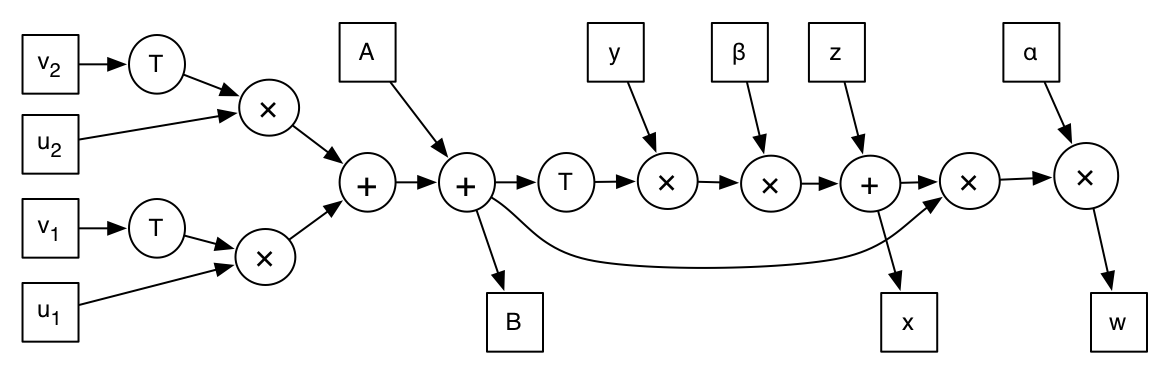
\includegraphics[width=3in]{figures/gemver-dataflow.png}
%\end{minipage}
%\caption{Dataflow graph (right) for the GEMVER kernel (left).}
%\label{fig:gemver-dataflow}
%\vspace{-.2in}
%\end{figure}

Here we briefly describe the analysis, refinement, and optimization of the
dataflow graph; these are discussed in more detail in~\cite{Siek}. 
During the analysis phase, all types of intermediate nodes are computed and
assigned. The algorithm choice and storage format determination are computed
simultaneously.  Consider, for example, the GEMVER kernel computation:   
$A \gets A + u_1 v_1^T + u_2 v_2^T;~
  x \gets \beta A^T y + z;~
  w \gets \alpha A x$.
The multiplication of $u_1$ and $v_1^T$ can be implemented by iterating over 
rows first or over columns first, depending on how the result is used
downstream in the dataflow graph.  In this case, the result is added to the
outer product of $u_2$ and $v_2^T$, so we still can choose either option as
long as we make the same choice for both outer products.
%Going one more step downstream, there is an addition with
%$A$, which was annotated in Figure~\ref{fig:gemver} to be column major. At
%this point it is clear that the outer-products should be computed in
%column-major order.

The information on implementation possibilities for basic linear algebra
operations is not hard-coded in the compiler; rather, this data is stored
in a database, called the \emph{linear algebra database}.  This separation
allows us to add new matrix formats, operations, and basic linear algebra
algorithms without changes to the compiler algorithm.

The analysis algorithm makes implementation choices using the
most-con\-strained-first strategy (also known as minimum remaining
values)~\cite{Russell:2003mz}.  The compiler chooses the node with the fewest
matching implementations (in the linear algebra database) and assigns an
algorithm name to the node.  If there is more than one match, the prototype
compiler picks the first.  This process is repeated with all remaining nodes
in the graph.

The refinement phase resolves the implementation for each operation node in
the graph into a subgraph defining the details of the chosen algorithm.  Each
subgraph is an abstract representation of the loop that implements the given
operation that also contains an iteration strategy for traversing the
elements of the matrix or vector.
In the optimization step, we apply conditional rewrite rules to optimize the
dataflow graph, for example merging two subgraphs when they share a common
operand. This rule is responsible for fusing the loops of the two
matrix-vector products in the GEMVER kernel.  
The final step performed by the MATLAB compiler when the graph cannot be
refined further is the generation of C code. The generator outputs a C loop
for each subgraph based on a topological sort of the graph. 

%Figure~\ref{fig:refine-mv-dot} shows two steps of refinement for a matrix-vector multiplication. The first step expands the matrix-vector multiplication according to the mv-dot algorithm: $(Ax)(i) = A(i,:)x$.  The refinement step replaces the $\times$ node with a subgraph that computes the inner product of a row of the matrix---the node labeled $(i,:)$---with the vector, storing the result in the $i$th element of the result vector---the node labeled $(i)$. The subgraph is labeled with $i=1\!:\!m$ indicating that the iteration strategy is to traverse the rows of the dense matrix.
%
%The second pass of refinement introduces another subgraph to implement the inner products. The new subgraph iterates through each dense row, as indicated by the $j=1:n$ annotation. The sign $\Sigma$ indicates that the sum of all of the iterations is computed.


%\begin{figure}[hbtp]
%  \centering
%  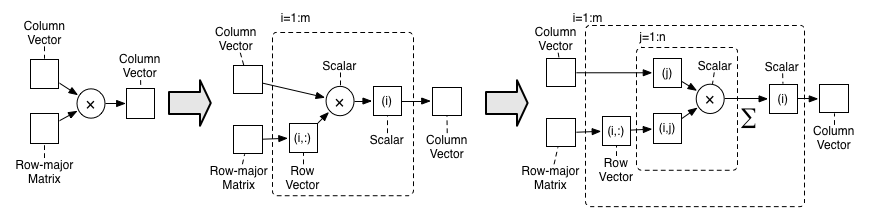
\includegraphics[width=\textwidth]{figures/refine-mv-dot.png}

%  \caption{The refinement of a matrix-vector product to a set of inner products and the refinement of inner products to scalar multiplications and additions.}
%  \label{fig:refine-mv-dot}
%\end{figure}

%\subsubsection{Optimize the Dataflow Graph.}



\subsection{Orio}
\label{sec:orio}

%~\cite{Norris:2007}
Orio\cite{Norris:2007,Hartono:IPDPS09} is an empirical tuning tool that takes
annotated C code as input, generates multiple transformed versions of the
annotated code, and empirically evaluates the performance of the generated
codes, ultimately choosing the best-performing version to use in production
runs.

Figure~\ref{fig:orio} illustrates the tuning process implemented in
Orio. The input to Orio is C code containing semantic comments that
describe both the computation (using a syntax that is more restricted
than the original C) and various performance-tuning directives. Orio
first extracts all annotation code regions by parsing the marked-up
input code. Each annotated region is then passed to code
transformation module and code generator for potential
optimizations. Next the transformed C code with various incorporated
optimizations corresponding to the specified annotations is
produced. Orio generates an optimized code version for each distinct
combination of performance parameter values. Each code
variant is then executed and its performance measured. After
iteratively testing all code variants, the best-performing code is
selected as the final output of Orio. While each variant is
computationally very cheap (a single code variant takes between a
fraction of a second to a few seconds depending on the input sizes),
the search space of all possible optimized code variants can be
exponentially large. Therefore, the search engine implements a number
of search heuristics (i.e., random, simplex, and simulated annealing)
to effectively narrow the search for near-optimal performance and
reduce the empirical search time. 
%The tuning
%specifications, written by users in the form of annotations, contains
%information required for guiding the transformation and tuning
%process.

\begin{figure}[tb]
%\vspace{-.3in}
\begin{center}
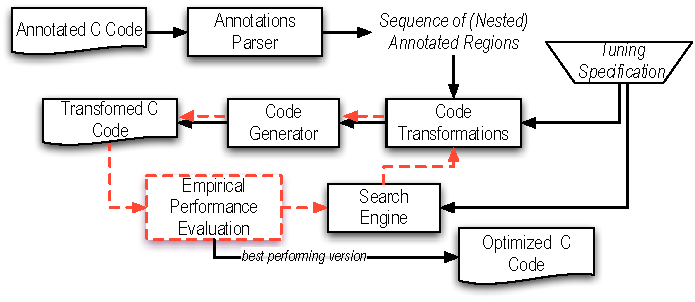
\includegraphics[width=.65\textwidth]{figures/orio.pdf}
\end{center}
\vspace{-.2in}
\caption{Overview of the Orio empirical tuning process.}
\label{fig:orio}
\vspace{-.15in}
\end{figure}

% --------------------------------------------------------------------------

\begin{figure}[htb]
\centering
\begin{tabular}{cc}
\begin{minipage}[b]{.45\textwidth}
\scriptsize
\begin{verbatim}
void vadd(int n, double *y, double *x1,
          double *x2, double *x3) {
/*@ begin PerfTuning(
  import spec vadd_tune_spec;
) @*/

 register int i;

/*@ begin BGP_Align(y[],x1[],
                    x2[],x3[]) @*/
/*@ begin Loop(
 transform Unroll(ufactor=UF, 
                  parallelize=PAR)
 for (i=0; i<=n-1; i++)
   y[i] = x1[i] + x2[i] + x3[i];
) @*/

 for (i=0; i<=n-1; i++)
   y[i] = x1[i] + x2[i] + x3[i];

/*@ end @*/
/*@ end @*/
/*@ end @*/
}

\end{verbatim}
\end{minipage}
&
\begin{minipage}[b]{.45\textwidth}
\scriptsize
\begin{verbatim}
spec vadd_tune_spec {
 def build { 
  arg build_command = 'mpixlc -O3 -qstrict -lm';
  arg batch_command = 'qsub -n 64 -t 10';
  arg status_command = 'qstat';
  arg num_procs = 64;
 }
 def performance_params { 
  param UF[] = range(1,32);
  param PAR[] = [True, False];
 } 
 def input_params { 
  param N = [10,100,1000,10**4,10**5,10**6,10**7];
 } 
 def input_vars {
  decl int n = N;
  decl double y[N] = 0;
  decl double x1[N] = random;   
  decl double x2[N] = random;   
  decl double x3[N] = random;   
 }
 def search {
  arg algorithm = 'Exhaustive';
 }
}
\end{verbatim}
\end{minipage}\\
\end{tabular}
\vspace{-.1in}
\caption{Orio example: Annotated C source code (left) and tuning specification excerpt for the Blue Gene/P (right).}
\label{fig:orio-example}
%\vspace{-.2in}
\end{figure}

Figure~\ref{fig:orio-example} shows an annotation example used by Orio to
empirically optimize VADD operation on Blue Gene/P. The annotations contain
performance hints that instruct Orio to perform memory alignment
optimization, loop unrolling, and multicore parallelization (using
OpenMP). In addition to these simple optimizations, Orio supports other
transformations such as loop blocking, loop permutation, scalar replacement,
array copy optimization, and some architecture-dependent optimizations. The
right-hand side of Fig.~\ref{fig:orio-example} shows separate tuning
specifications used for building and running executable tests, including
performance parameter values, execution environment details, input variable
information, and the search algorithm. Orio also supports parallel search
when parallel resources are available. In this example, the parallel Orio
driver simultaneously executes 64 code variants in the same parallel job. 
%The
%commands used by Orio to submit a parallel job and to query its status are
%also specified in the tuning specifications. 
At present, users must create the tuning specifications manually for
each architecture. When Orio is used in conjunction with compiler
tools, such as the MATLAB compiler described in this paper, it should
eventually be possible to automatically generate the tuning
specifications.

%\vspace{-0.1in}

\section{Experimental Results}
\label{sec:experiments}

We evaluated our approach by running experiments on an Intel Xeon
workstation and the Blue Gene/P at Argonne. The Intel machine has dual
quad-core E5462 Xeon processors (8 cores total) running at 2.8 GHz
(1600 MHz FSB) with 16 GB RAM, running Ubuntu 8.04. Intel C compiler
(v10.1) was used with \texttt{-O3} option (and
\texttt{-parallel}/\texttt{-openmp} for automatic/manual
parallelization, respectively). Each node of the Blue Gene/P has four
850 MHz PowerPC 450 processors with a dual floating-point unit and 2
GB total memory per node, running a proprietary operating system. On the
Blue Gene/P, we used IBM XLC compiler (v9.0), with \texttt{-O3
-qstrict -qarch=450d -qtune=450 -qhot} options (and
\texttt{-qsmp=auto}/\texttt{-qsmp=noauto} for automatic/manual
parallelization, respectively).

Table~\ref{tbl:blas-ops} lists the composed BLAS operations used in our
experiments, along with their input and output variables. Vectors are typeset
in lowercase with an overhead arrow. Scalars and matrices are represented as
lowercase and uppercase letters, respectively. A regular uppercase denotes a
row matrix, whereas a bold uppercase symbolizes a column matrix. The extended
MATLAB expression that corresponds to each operation can be seen in the last
column of Table~\ref{tbl:blas-ops}.


\begin{table}[htb] 
%\vspace{-.1in} 
\caption{Composed BLAS operations used in our experiments.}
\label{tbl:blas-ops}
\small
\centering 
%\vspace{-.1in} 
\begin{tabular}{c c c c} 
\hline 
Name & Input & Output & Operation  \\ 
\hline 
%\hline 
%& & & \\
VADD & $\overrightarrow{w}$,$\overrightarrow{y}$,$\overrightarrow{z}$ & $\overrightarrow{x}$ &
$\overrightarrow{x} = \overrightarrow{w} + \overrightarrow{y} + \overrightarrow{z}$ \\ [1ex]
%---------------------------------------------------------------------------------
%\hline 
%& & & \\
ATAX & $A$,$\overrightarrow{x}$ & $\overrightarrow{y}$ & 
$\overrightarrow{y} = A^T * (A * \overrightarrow{x})$ \\ [1ex]
%---------------------------------------------------------------------------------
%\hline 
%& & & \\
GEMVER & ${\bf A}$,$a$,$b$, &  ${\bf B}$,  & ~~${\bf B} = {\bf A} + \overrightarrow{u_1} * \overrightarrow{v_1}^T + \overrightarrow{u_2} * \overrightarrow{v_2}^T$\\
 & $\overrightarrow{u_1}$,$\overrightarrow{u_2}$,$\overrightarrow{v_1}$,$\overrightarrow{v_2}$, & $\overrightarrow{x}$,$\overrightarrow{w}$ & $\overrightarrow{x} = b * ({\bf B}^T * \overrightarrow{y}) + \overrightarrow{z}$\\
& $\overrightarrow{y}$,$\overrightarrow{z}$ &  & $\overrightarrow{w} = a * ({\bf B} * \overrightarrow{x})$\\ [1ex]
%---------------------------------------------------------------------------------
%\hline 
BiCG Kernel & ${\bf A}$,$\overrightarrow{p}$,$\overrightarrow{r}$ & $\overrightarrow{q}$,$\overrightarrow{s}$ & $\overrightarrow{q} = {\bf A} * \overrightarrow{p}$ \\ 
& & & $\overrightarrow{s} = {\bf A}^T * \overrightarrow{r}$\\
 
\hline 
\end{tabular} 
\vspace{-.1in} 
\end{table} 


\begin{figure}[htp]
{\small
\centering
\begin{tabular}{cc}

\begin{minipage}[b]{.5\textwidth}
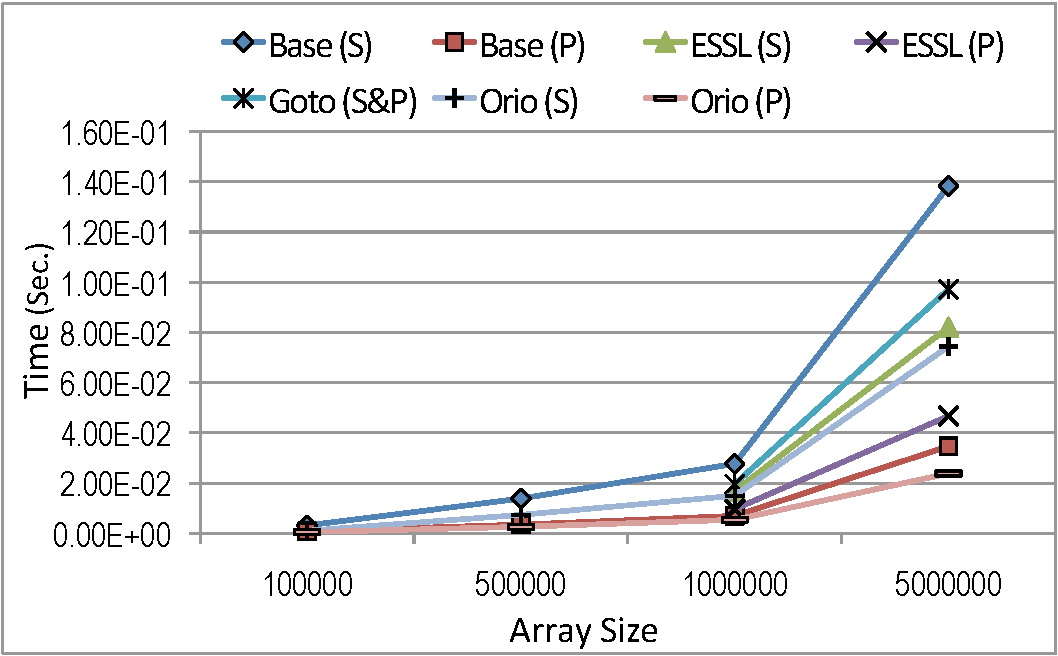
\includegraphics[width=\textwidth]{figures/vadd_bgp_time2.pdf}
\end{minipage}
&
\begin{minipage}[b]{.5\textwidth}
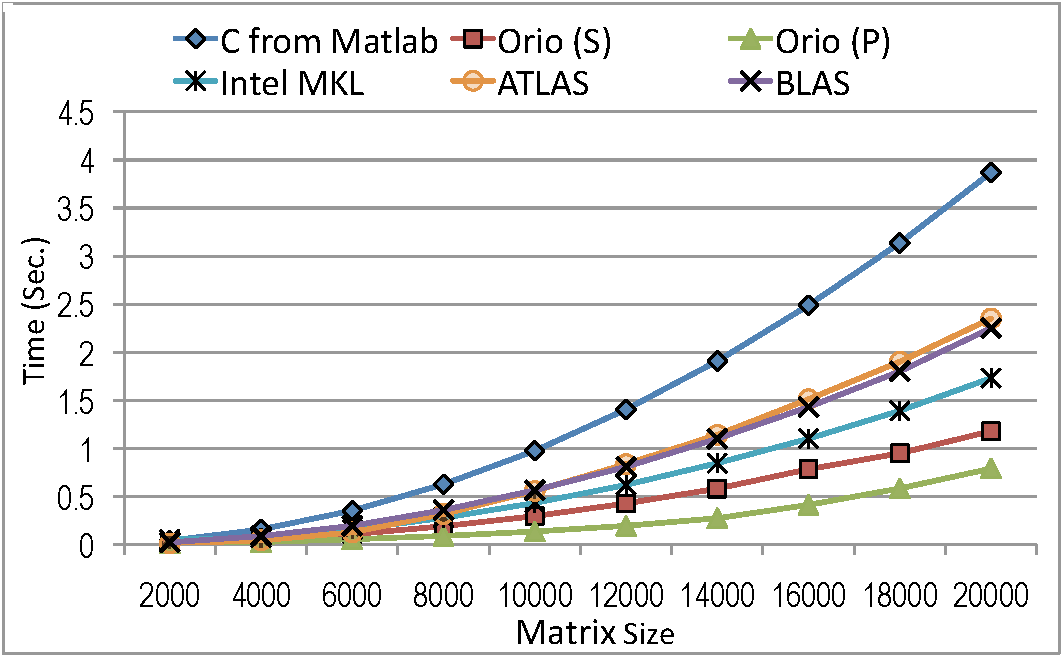
\includegraphics[width=\textwidth]{figures/atax.pdf}
\end{minipage}\\

(a) VADD & (b) ATAX \\

\begin{minipage}[b]{.5\textwidth}
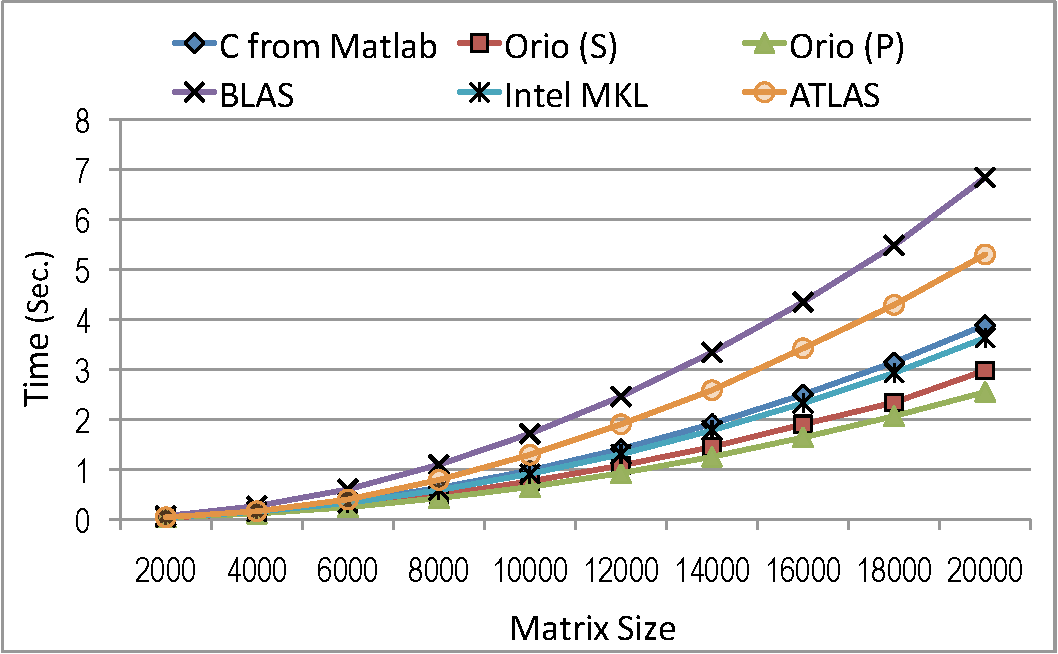
\includegraphics[width=\textwidth]{figures/gemver.pdf}
\end{minipage}
&
\begin{minipage}[b]{.5\textwidth}
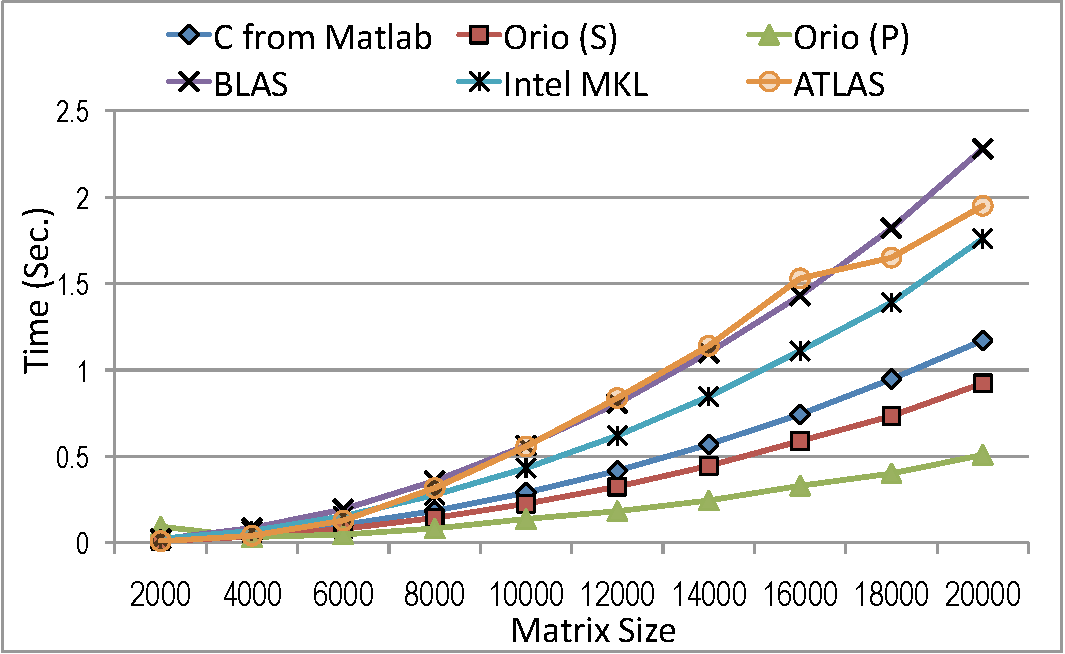
\includegraphics[width=\textwidth]{figures/bicgkernel.pdf}
\end{minipage}\\

(c) GEMVER & (d) BiCG Kernel \\

\end{tabular}
}
\vspace{-.1in}
\caption{Performance results for several composed BLAS operations.}
\label{fig:results}
\vspace{-.1in}
\end{figure}

The performance results of tuning the VADD operation on the Blue
Gene/P are given in Fig.~\ref{fig:results}(a). The ``Base'' label
designates the C implementation generated by the MATLAB compiler. We also
tested the performance of an implementation that calls
\texttt{DAXPY} twice using available BLAS libraries.
Finally, we tuned the simple C loop version using Orio, with the performance
annotations previously shown in Fig.~\ref{fig:orio-example}. In this
experiment, we measured the performance for both the sequential and parallel
scenarios (indicated by (S) and (P) in the legend, respectively). Even for a very simple operation such as vector addition the
compiler alone is unable to obtain the same level of performance as the
empirically tuned versions. Furthermore, as expected, the BLAS implementation
does not exploit locality and thus performed worse than the single-loop
implementation.
%of the single loop implementation due to l
% however, selecting the correct compiler
%options was crucial for achieving good performance of the base version.

The experiments of the remaining operations were performed on the
multicore Intel Xeon. Included in these experiments are performance
numbers for six code variants: the C code generated by the MATLAB
compiler (``C from MATLAB''), three BLAS-based implementations that
use Intel MKL, ATLAS, and the default BLAS library on Ubuntu 8.04, and
the sequential and parallel code variants tuned by Orio (``Orio
(S)'' and ``Orio (P)'', respectively).

The Xeon performance results of ATAX are shown in
Fig.~\ref{fig:results}(b). The Orio-tuned version that incorporates
Pluto-generated loop fusion optimizations and Orio parallelization
directives achieves the best performance for most problem sizes,
outperforming the Intel MKL version by a factor of 2 to 5.7 and the
compiler-optimized C version by a factor of 4 to 7. The optimizations
performed by both Orio versions include scalar replacement,
vectorization, and loop unroll/jam.

Figure~\ref{fig:results}(c) shows the performance of the GEMVER
operation on the Xeon workstation. Here we used the same Pluto and Orio
optimizations as for the ATAX example. Similarly, the parallel Orio version
achieved the best performance, although in this case the sequential Orio
version performs almost the same, suggesting that the compiler was not able
to parallelize the code very effectively. For this operation, substantial
performance differences exist between among the different BLAS versions, with
the Intel MKL version achieving performance close to that of the simple
compiler code.

The performance for the BiCG kernel operation is shown in
Fig.~\ref{fig:results}(d). For this operation, the Pluto analysis did not
result in performance improvement. Thus we are showing the results obtained
only through Orio transformations, which included vectorization, scalar
replacement, and loop unroll/jam. Again the best performance was achieved
by the parallel Orio version, while all the BLAS versions performed worse
than the compiler-optimized C loop version.

\section{Conclusions}
\label{sec:conclusion}

We have described an approach to generating tuned linear algebra libraries
from high-level annotated MATLAB code that involves a suite of tools to (1)
translate the MATLAB code to C, (2) analyze the resulting loops and identify
locality and parallelism-enhancing optimizations using Pluto, and (3)
annotate the resulting C code with syntactic performance directives and use
Orio to generate multiple optimized versions and empirically select the one
with the best performance. Preliminary results from experiments with several
composed BLAS operations show that the optimized code generated by this suite
of tools significantly outperforms the versions using tuned BLAS and
aggressive compiler optimizations.

The positive initial results from our approach to generating tuned linear
algebra routines motivate several future lines of investigation, including closer
integration between the tools handling the different steps of the process and 
more automation at each step.
%At present
%there are a number of manual steps involved in obtaining a compiled tuned
%linear algebra library from the high-level extended MATLAB descriptions. We
%will work on the more close coupling of our separately developed tools and
%fully automating their interactions. This would enable application developers
%to easily produce custom linear algebra libraries tuned for specific
%architectures.

% We will also investigate extending the supported functionality
%of our MATLAB compiler beyond composed BLAS operations, thus benefiting a
%wider spectrum of applications.

%Orio is growing in a number of directions. While it automates much of the
%tuning process, a number of steps still require nontrivial manual
%input. Orio's modular design allows new transformations to be added easily,
%which presents many opportunities for expanding the existing set of
%optimizations with new ones implemented from scratch or through interfaces to
%other tools, as we have successfully done with Pluto. We are also working on
%generating code that contains special cases for different input parameter
%values since in many cases different optimizations are optimal for different
%input sizes.  We will also continue developing the parallel empirical search
%infrastructure; it is clear that more feedback between the MATLAB compiler
%and Orio will result in automation of the performance directive annotation
%process and a much more effective exploration of the search space. We plan to
%use a fast analytic cost function in the MATLAB compiler implementation to
%prune out regions of the search space that will not produce competitive
%implementations. The cost function is based on a model of the computer
%architecture, but does not necessarily account for all the details. Once the
%search space is narrowed, we will use the Orio empirical testing results with
%representative data sets to determine the exact performance of the
%alternatives and choose the best one.

%Finally, while Orio currently generates various loop transformations, it does
%not generate calls to existing library implementations. For this paper, we
%implemented the BLAS versions of all operations manually. Our past success
%with identifying Blue Gene/L intrinsics from expression graphs motivate
%further research on identifying BLAS and other established library operations
%from the expression graphs of the MATLAB code.

%\singlespacing
%% or stuff it in a footnote
%\section*{Acknowledgments}
%This work was supported by the Mathematical, Information, and
%Computational Sciences Division subprogram of the Office of Advanced
%Scientific Computing Research, Office of Science, U.S. Dept. of Energy,
%under Contract DE-AC02-06CH11357. 
%TODO: need Colorado and Ohio acknowledgments

\nopagebreak
\bibliographystyle{splncs}
\bibliography{paper}


%\newpage
%\vfill
%\begin{flushright}
%\scriptsize
%\framebox{\parbox{2.4in}{The submitted manuscript has been created by
%UChicago Argonne, LLC, Operator of Argonne National Laboratory
%("Argonne").  Argonne, a U.S. Department of Energy Office
%of Science laboratory, is operated under Contract No.
%DE-AC02-06CH11357.  The U.S. Government retains for itself, and
%others acting on its behalf, a paid-up, nonexclusive, irrevocable
%worldwide license in said article to reproduce, prepare derivative works,
%distribute copies to the public, and perform publicly and display
%publicly, by or on behalf of the Government.}}
%\normalsize
%\end{flushright}

\end{document}
